\section{Calibration Campaigns}\label{sec:CalibCampaigns}
\subsection{Radioactive Sources}
For calibration of \lsv\ detector response and \tpc's response to electron recoils (ER) $^{57}$Co, $^{133}$Ba and $^{137}$Cs were selected. $^{22}$Na was deployed in a later calibration campaign. They allow a cross-calibration with $^{83m}$Kr injected in Argon recirculation system during dedicated campaigns and internal $^{39}$Ar, as they cover the $^{39}$Ar energy range (see also Table~\ref{tbl:GammaSources} and Fig.~\ref{fig:GammaSources_Ar39spectrum}). %As the interaction length increases with energy in LAr, the different gamma sources allow also to probe different regions of the TPC active volume.  

After a gamma source energies preselection, detailed studies with DarkSide Monte Carlo simulation package G4DS \cite{DS50:G4DS:paper} were performed to select appropriate source activities and check various deployment positions' feasibility and physics reach. Sources with suitable activities were identified for deployment considering also constraints from \lsv\ and \tpc\ DAQs (Table~\ref{tbl:GammaSources}).

Energy variables are calibrated in photo-electrons (PE) using dedicated laser calibration runs, in which each PMT's single PE charge spectra are fitted and a PE-charge gain is determined. 
These laser runs are also an integral part of a calibration campaign requiring a laser run every few hours and at least on each change in DAQ, \tpc\ or CALIS configuration, such as drift field changes or source position changes.

\begin{figure}[htbp]
 \centering
 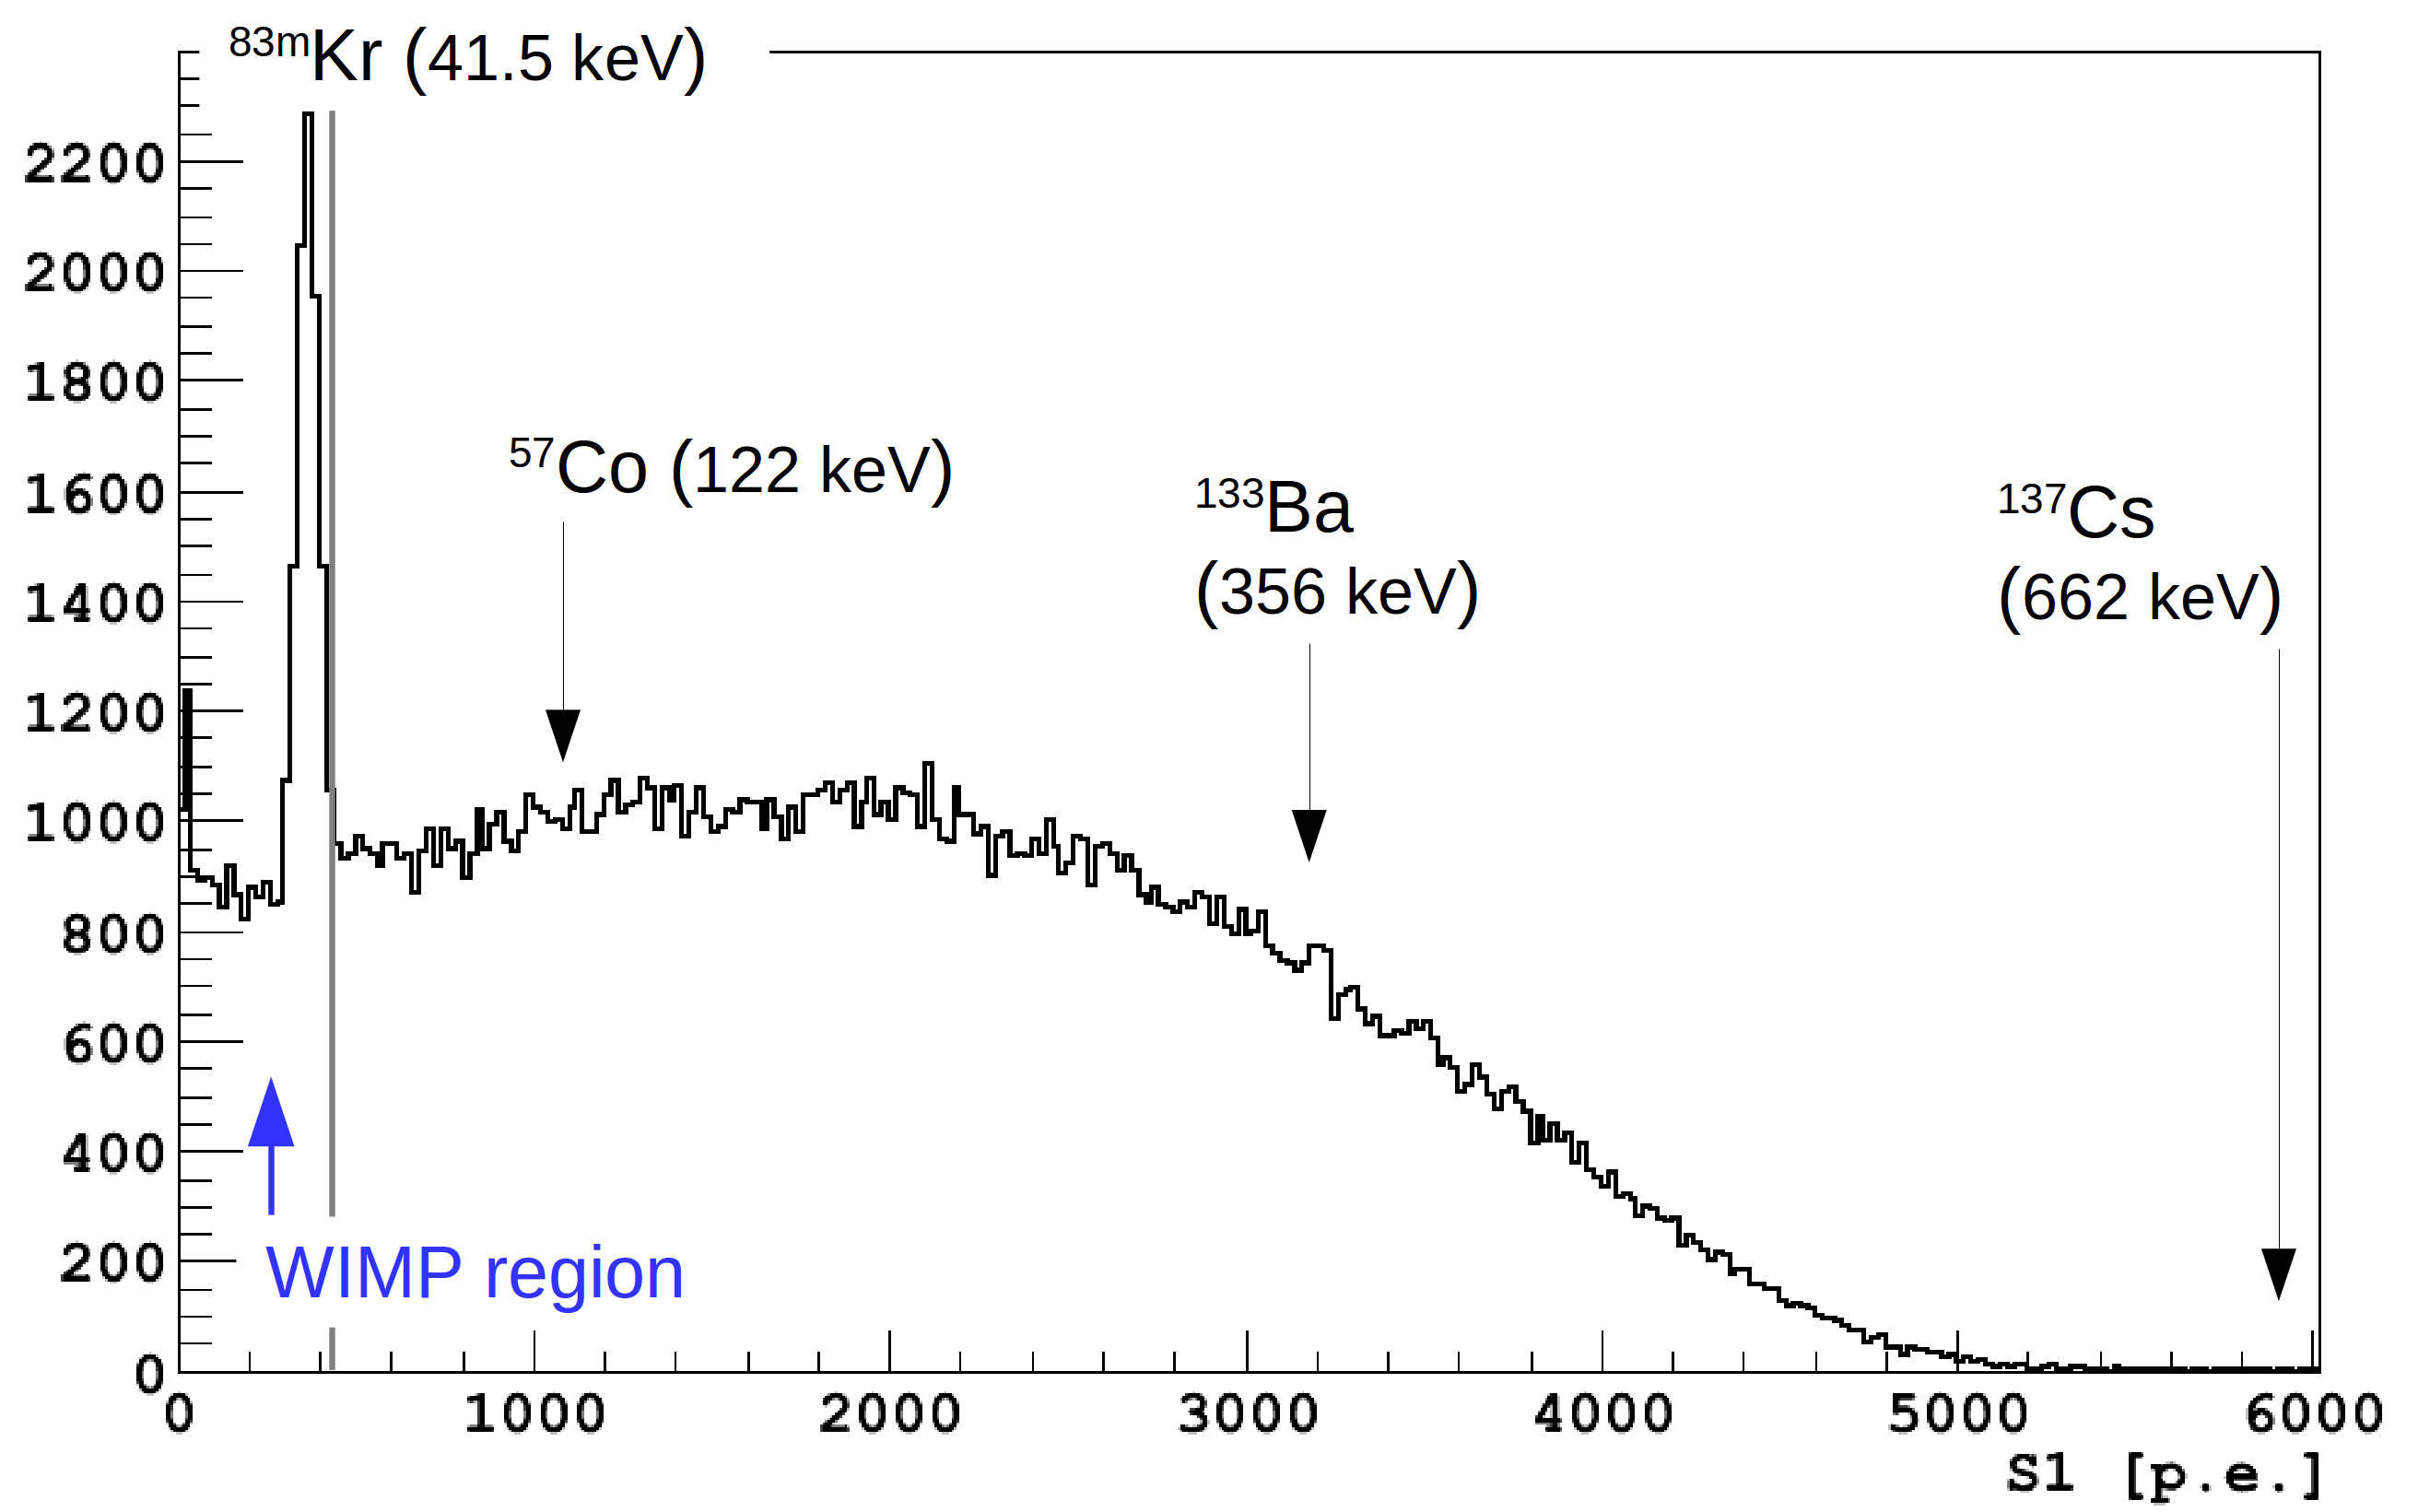
\includegraphics[width=0.8\textwidth]{Figures/GammaSources_Ar39spectrum.png}
 \caption{Scintillation spectrum (S1) at null field showing a $^{83m}$Kr peak on internal $^{39}$Ar $\beta$ spectrum. Positions of full absorption peaks of three gamma sources are indicated and cover $^{39}$Ar spectrum's full range.
\label{fig:GammaSources_Ar39spectrum}}
\end{figure}

\begin{table}[htbp]
\centering
\caption{Gamma sources deployed in DS-50, $^{39}$Ar and $83m$Kr \cite{Lippincott:2010jb}. $^{39}$Ar activity has been approx. 50 Bq (1 Bq/kg) during AAr filling and negligible in the UAr phase. The Kr source activity varied from campaign to campaign, but was in range of a few Bq to some tens of Bq.} %\cite{Lippincott:83mKr}
\centering
\begin{tabular}{|l|l|l|l|l|}
\hline
\textbf{source} & \textbf{type} & \textbf{energy} & \textbf{half life} & \textbf{activity} \\ \hline
$^{57}$Co & $\gamma$ & 122 keV & 0.744 y  & 35 kBq \\ \hline
$^{133}$Ba & $\gamma$ & 356 keV & 10.54 y & 2 kBq \\ \hline
$^{137}$Cs & $\gamma$ & 662 keV & 30.2 y & 0.65 kBq \\ \hline
$^{22}$Na & $\gamma$ & $2\cdot 511$ keV + 1274 keV & 2.603 y & 11 kBq \\ \hline\hline
$^{39}$Ar & $\beta$ &  565 keV endpoint& 269 y  & 50 Bq\\ \hline
$^{83m}$Kr & 2 $\beta$ &  32.1 keV + 9.4 keV & 86.2 d & varying\\ \hline
\end{tabular}
\label{tbl:GammaSources}
\end{table}

%\begin{tabular}{|l|l|l|l|l|l|}
%\hline
%\textbf{source} & \textbf{type} & \textbf{energy} & \textbf{half life} & \textbf{interact. length} & \textbf{activity} \\ \hline
%$^{57}$Co & $\gamma$ & 122 keV & 0.744 y & 4.4 cm & 35 kBq \\ \hline
%$^{133}$Ba & $\gamma$ & 356 keV & 10.54 y & 7.5 cm & 2 kBq \\ \hline
%$^{137}$Cs & $\gamma$ & 662 keV & 30.2 y & 9.5 cm & 0.65 kBq \\ \hline
%$^{22}$Na & $\gamma$ & $2\cdot 511$ keV + 1274 keV & 2.603 y & 8.4/ 11.3 cm & 11 kBq \\ \hline\hline
%$^{39}$Ar & $\beta$ &  565 keV endpoint& 269 y & sub-mm & 50 Bq\\ \hline
%$^{83m}$Kr & 2 $\beta$ &  32.1 keV + 9.4 keV & 86.2 d & sub-mm & varying\\ \hline
%\end{tabular}
%\label{tbl:GammaSources}


\subsection{Calibration Campaigns Timeline and Stability}
Following calibration campaigns were performed between October 2014 and April 2016:
\begin{itemize}
\item First extensive campaign involving all gamma sources and both high and low activity AmBe neutron source took place in October and November 2014 at LNGS. \tpc\ was filled with Atmospheric Argon  with an inherent trigger rate of approx. 50 Hz from $^{39}$Ar. \lsv\ liquid scintillator consisted of PC only with $<0.1 \%$ TMB and 1.4 g/l PPO as wavelength shifter.
%Fig.~\ref{???} shows the different configurations in which data has been taken as a function of source energy, source position and drift field.

\item In January and February 2015 a second campaign focusing on \lsv\ calibration using low activity AmBe source was performed. Before this \lsv\ was reconstituted with 5\% TMB. Two deployments were performed at two different PPO concentrations (0.7 g/l and 1.4 g/l), allowing to study PPO concentration impact on alpha and gamma quenching. (1.4 g/l is our nominal PPO concentration, see also Fig.~\ref{fig:LSV:Calib}, right)

\item In August 2015 a $^{22}$Na source was deployed next to cryostat for TPC calibration. This was first gamma source calibration campaign after UAr deployment within \dsf.
\item In December 2015 an $^{241}$Am$^{13}$C neutron source has been deployed, allowing an in-depth study of detection efficiency of prompt neutron recoil signal in absence of correlated 4.4 MeV gamma, obfuscating neutron recoil signal in case of an AmBe source.
\end{itemize}

In dedicated analyses it has been shown that calibration campaigns have not affected negatively light yield or introduced radioactivity into the LSV \cite{Agnes:2015qyz}.

%\begin{figure}[htbp]
%\centering
%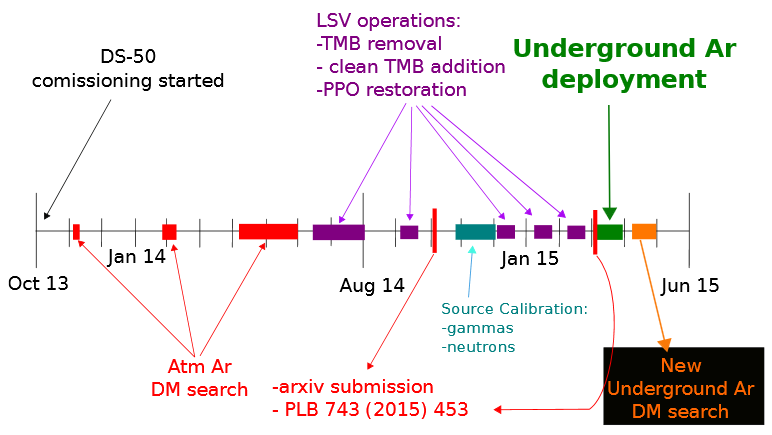
\includegraphics[width=0.7\textwidth]{./Figures/Yann_timeline.png}
%\caption{In black the stability of the LSV LY is monitored using internal $^{60}$Co emitted from the cryostat steel, in blue the stability %of the rate of radioactivity in the LSV is shown. Before and after calibration campaigns both the LY and the rate remain unaffected.
%\label{fig:LSV:Stability}}
 %\end{figure}


\subsection{TPC Calibration}
A few calibration results are shown illustrating acquired calibration data quality and their description in G4DS.

\subsubsection{$^{57}$Co S1 energy}
Fig.~\ref{fig:CalibData:Co57} shows a data-MC comparison of scintillation signal S1 spectrum of a $^{57}$Co calibration source deployed next to cryostat and close to TPC active volume center. S1 distribution is overlayed by an equivalent selection of G4DS MC simulation events.\mymarginpar{The plot is from Paolo's G4DS talk \@ DS2016, UCLA. Ideally one could get an official copy from the MC paper.}

\begin{figure}[htbp]
\centering
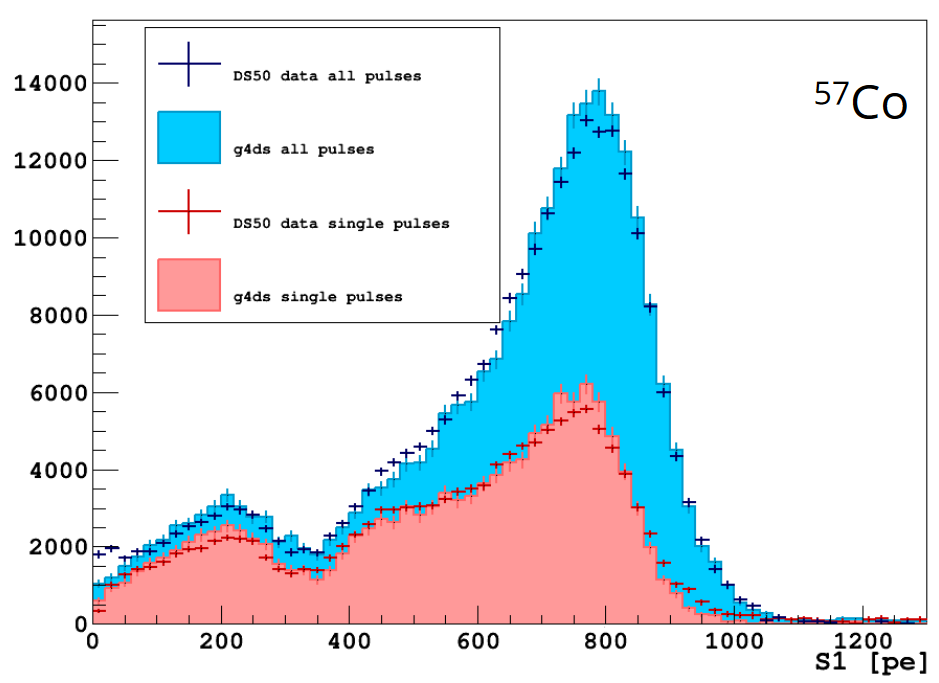
\includegraphics[width=0.7\textwidth]{./Figures/57Co_Paolo_G4DS_UCLA.png}
\caption{Data-MC comparison for $^{57}$Co source deployed next to cryostat. In magenta distribution a single-site interaction requirement is imposed as for dark matter events and for blue distribution this constraint is removed \cite{DS50:G4DS:paper}.
\label{fig:CalibData:Co57}}
 \end{figure}


\subsubsection{F90 distribution from $^{241}$Am$^9$Be neutron data}\label{sec:CalibData:NR}

Fig.~\ref{fig:CalibData:F90} shows good agreement between F90 medians and S1 spectra measured from $^{241}$Am$^9$Be neutron data and those derived from \SCENE\ measurements, which have been used to determine nuclear recoil energy scale and NR acceptance regions for WIMP dark matter search \cite{Agnes:2015gu, Agnes:2015_uar}.
\begin{figure}[htbp]
\centering
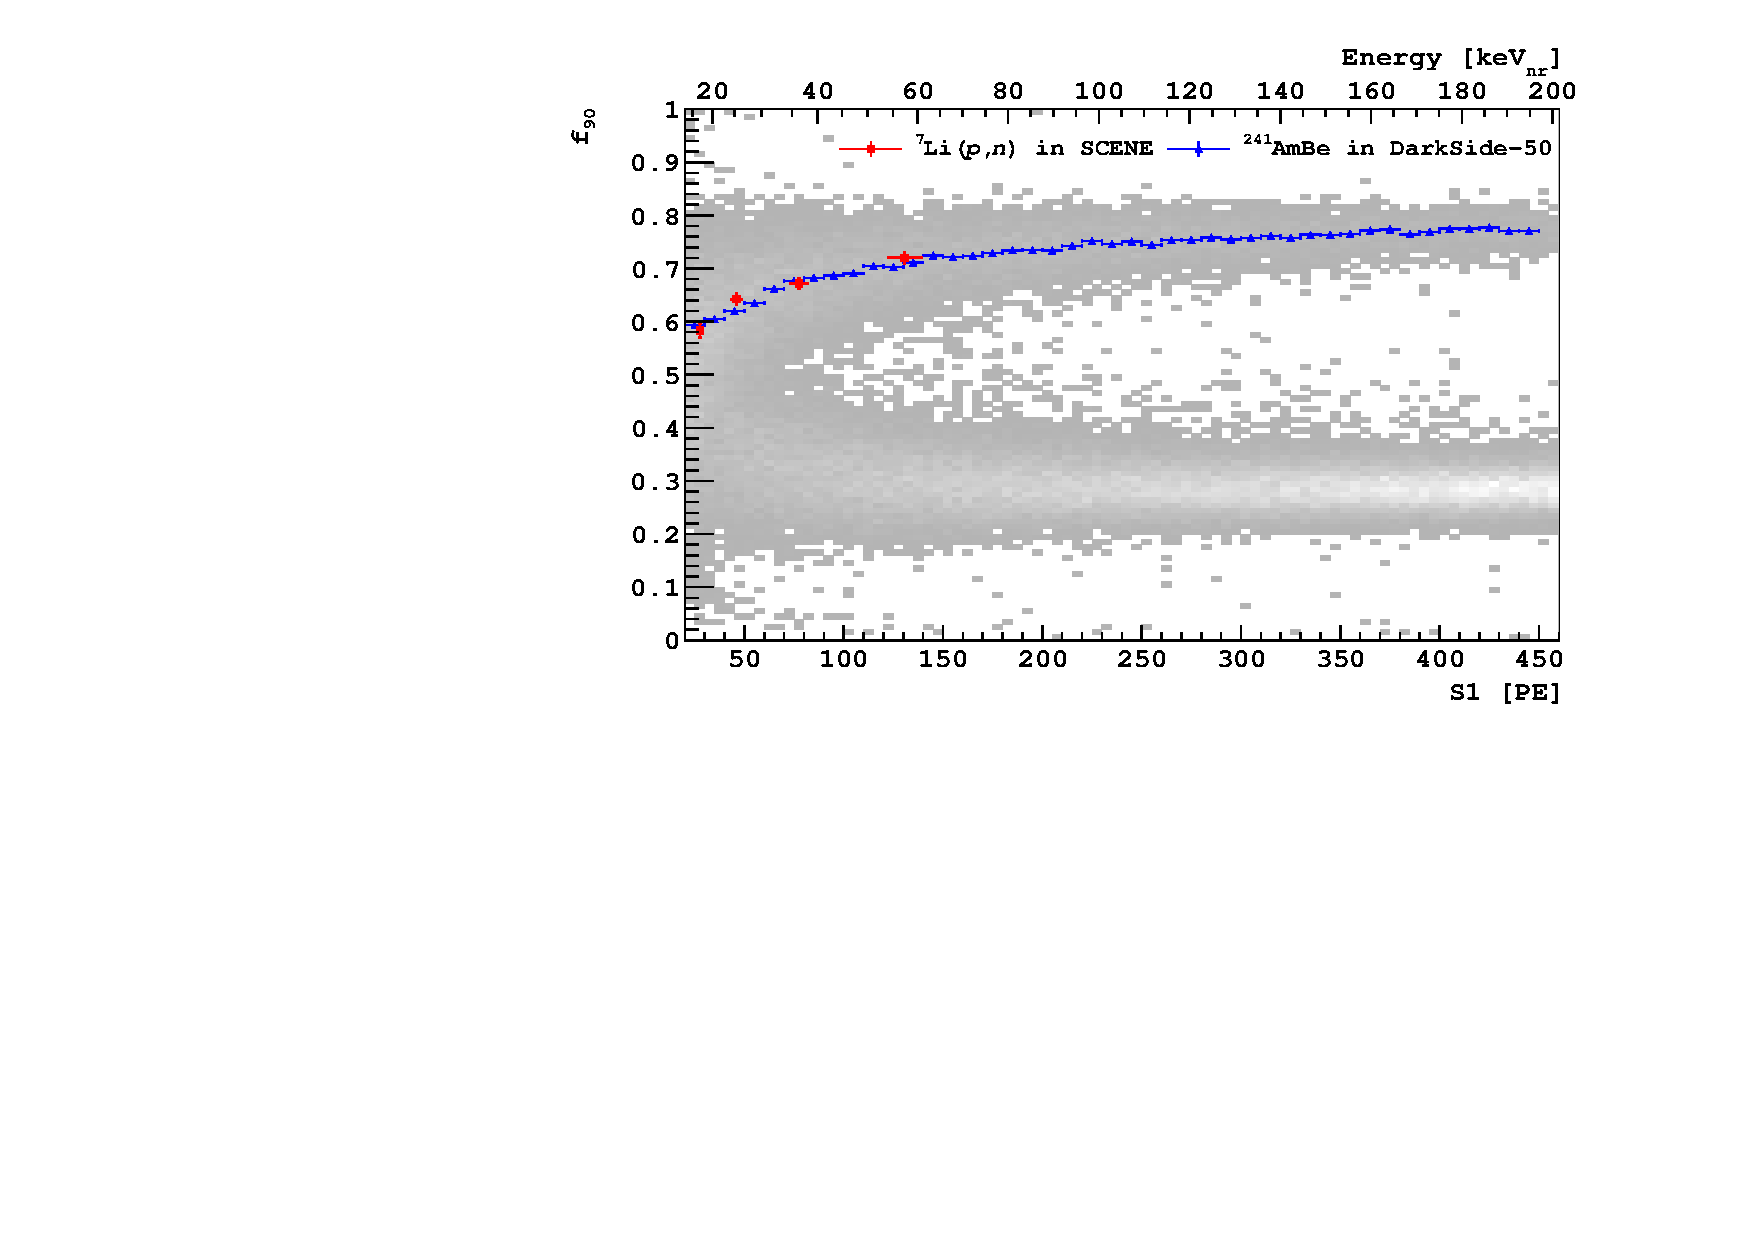
\includegraphics[width=0.7\textwidth]{./Figures/DSf-UArAmBeDMSStCut.pdf}
\caption{Plot of F90 vs. scintillation signal S1 from a high rate AmBe neutron source calibration of \dsf\ in grey, upper NR band from AmBe calibration and lower ER band from $\beta$-$\gamma$ backgrounds are visible. Overlaid are \FNinety\ \NR\ median vs. \SOne\ from a high-rate {\it in situ} AmBe\ calibration (blue) and scaled from \SCENE\ measurements (red points) \cite{Cao:2015ks}. There is very good agreement between the two.  High source intensity and correlated neutrons and $\gamma$-ray emission by AmBe source contribute events outside nuclear recoil and electron recoil bands. (reproduced from \cite{Agnes:2015_uar})\label{fig:CalibData:F90}\label{fig:DSf-UArAmBeDMS}} 
\end{figure}


\subsubsection{Source position}
Tests at LNGS established the deployment system's positioning accuracy to be about $\pm$1 cm after a 7 meter journey into the \dsf\ \lsv.
%comment to the "about $\pm ": the tilde $~ \pm$ did not show up at all in the output.
During first calibration campaign several runs have been taken with source at its central position (731000 motor step counts). Fitting t$_{drift}$ distribution at that position for a sequence of runs a systematic shift vs.~time has been observed (Fig.~\ref{fig:SourcePosition}, right). The source position has been on average 157.4 mm below the grid with an RMS of 10.1 mm. Following that observed systematic shift with time deployment procedures were revised to avoid such a time dependency in the future and to improve the deployment precision: Prior to moving source to its target position, deployment device is sent to its lowest position, where cables are fully unwound and any build-up in the cables is released. It is worth mentioning this does not induce significant uncertainties for calibration data analyses, as t$_{drift}$ distribution can be measured in-situ on a per-run basis and hence does not affect our dark matter analysis.
\begin{figure}[htbp]
\centering
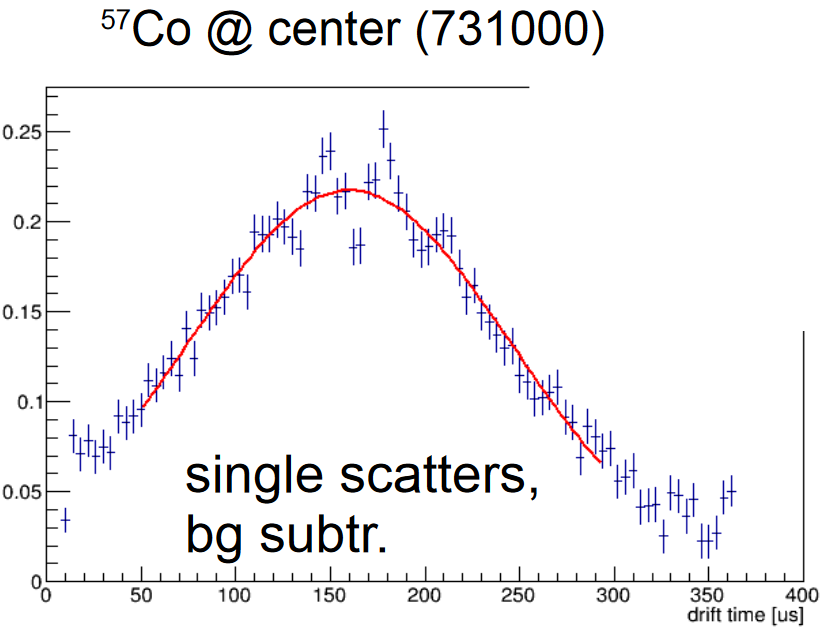
\includegraphics[width=0.48\textwidth]{./Figures/Tdrift_distribution_Co57_DocDB1288.png}
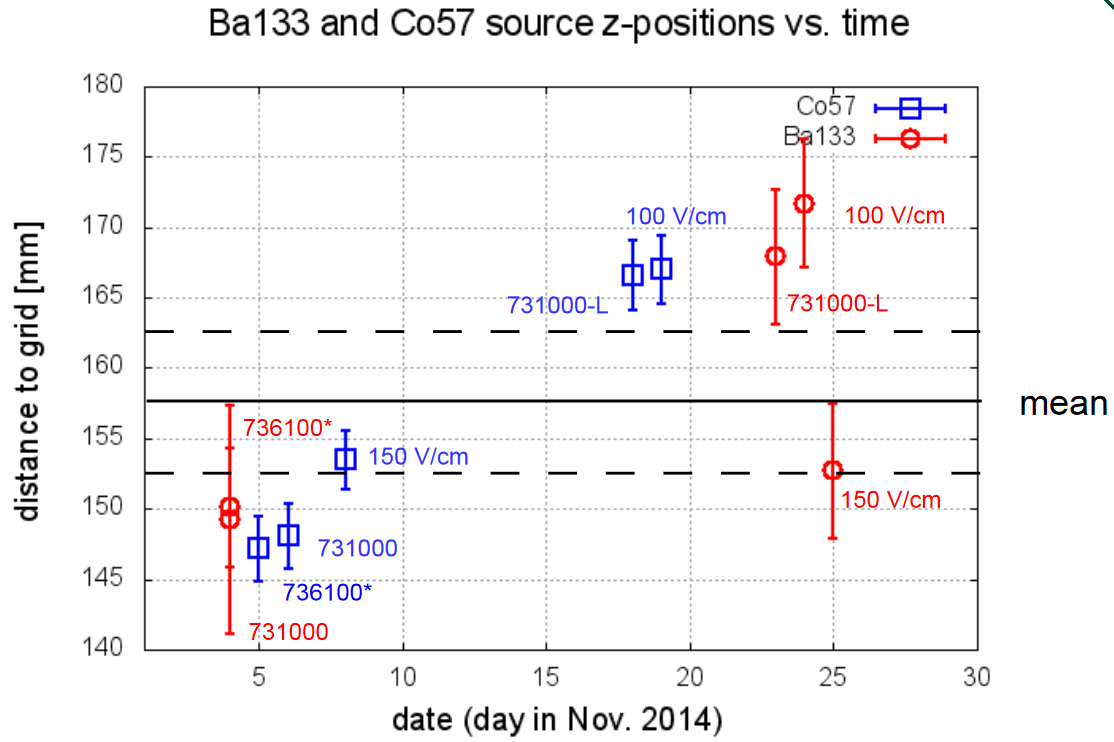
\includegraphics[width=0.48\textwidth]{./Figures/SourcePosition_vs_time_DocDB1288.png}
\caption{\textit{left:} A t$_{drift}$ distribution encoding the Z-position of $^{57}$Co deployed next to TPC vertical center.
\textit{right:} Shift of source position relative to TPC grid as a function of time when deployed to same place.
\label{fig:SourcePosition}} 
\end{figure}

For XY-position azimuthal angle distribution in XY-plane has been studied and a 139 degree mean was observed with a 1.2 deg RMS. (One degree corresponds to 6 mm at the outer cryostat, where source is positioned.) However an independent XY reconstruction algorithm gave 142.5 degrees with an 0.8 deg RMS, so that systematic uncertainties from reconstruction dominate over XY precision. %\cite{DS:XY:paper}.
\mymarginpar{This is from DocDB 1288. Ideally one could cite a XY paper here, which is not published yet.}


%%%%%%%%%%%%%%%%%%%%%%%%%%%%%%%%

\subsection{Liquid Scintillator Veto}\label{sec:LSV:gammasources}

In Fig.~\ref{fig:LSV:Calib} (left) a data-MC comparison of LSV charge spectra from a $^{137}$Cs source deployed in LSV next to cryostat is shown \cite{DS50:G4DS:paper}.
In January and February 2015 LSV scintillator reconstitution was completed and a second LSV calibration using AmBe neutron source was undertaken to further study various LSV neutron detection channels. With a borated scintillator, a critical aspect of neutron detection efficiency is the capability to observe \brbortenground\ capture branch leading to a \enbortengroundalpha\ $\alpha$ + $^7$Li(g.s.) without accompanying 478 keV $\gamma$-ray. As shown in Fig.~\ref{fig:LSV:Calib} (right) the de-excitation channel is clearly observed at around 30 PE.

\begin{figure}[htbp]
\centering
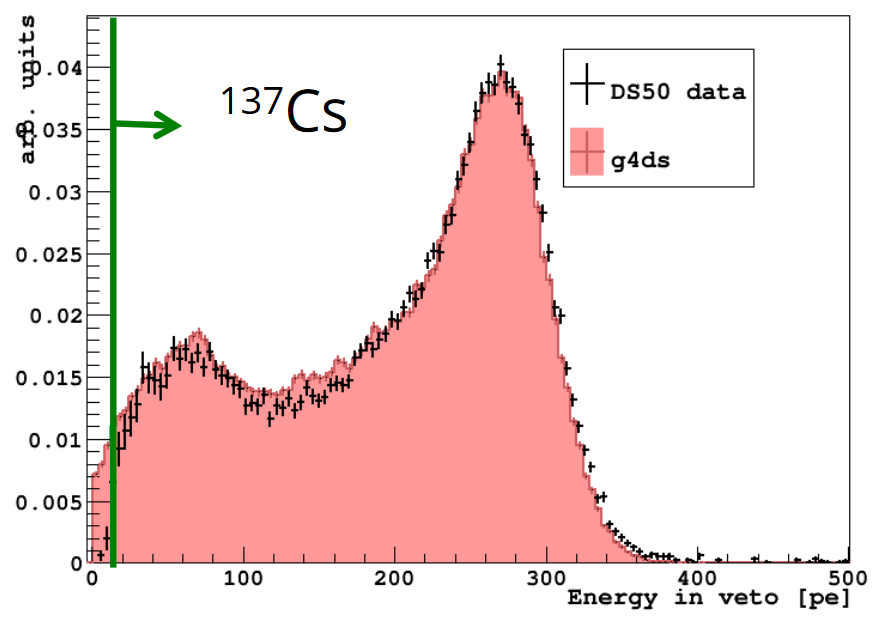
\includegraphics[width=0.48\textwidth]{./Figures/137Cs_Veto_Paolo_G4DS_UCLA.png}
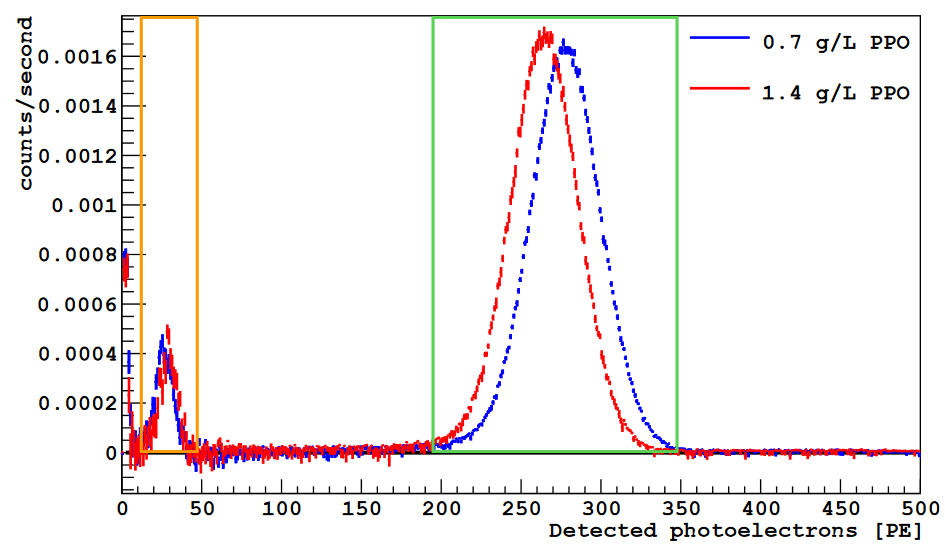
\includegraphics[width=0.48\textwidth]{./Figures/AmBe_LSV_VetoPaper.png}
\caption{\textit{left:} LSV charge spectra data-MC comparison from $^{137}$Cs source deployed in LSV next to the cryostat \cite{DS50:G4DS:paper}.
\textit{right:} Clear neutron capture signal detection on $^{10}$B in LSV leading to a \enbortengroundalpha\ $\alpha$ + $^7$Li(g.s.) at $\approx$ 30 PE (orange box). Peak on the right at $\approx$ 270 PE (green box) is from 93.6 \% of captures that lead to the $^7$Li excited state reaction, with the accompanying 478 keV-ray. The entries below 10 PE are due to PMT after-pulses. Data has been taken before and after varying PPO wavelength shifter concentration in the scintillator with the source rotated 70 cm away from the cryostat. In both cases the deexcitation to ground state is clearly observed.\cite{Agnes:2015qyz}
\label{fig:LSV:Calib}} 
\end{figure}